\documentclass{article} %[letterpaper,11pt]
\usepackage{graphicx}
\usepackage{caption}
\usepackage{subcaption}
\usepackage{url}

\usepackage{amsmath}

\newcommand{\code}[1]{\texttt{#1}}
\renewcommand\refname{7  \hspace{4 mm}References}

\begin{document}

\title{CS 867: Exploring Alternatives to Line Charts}
\date{October 20, 2013}
\author{Carmen St.\ Jean}

\maketitle

\section{Introduction}

Since its introduction in 1786 by Playfair \cite{playfair1786}, the line chart has been the conventional choice for visualization of temporal data in different fields such as medicine, economics, and ecology.  Though line charts are quite popular, perhaps alternatives might be better suited for depicting time-oriented data in an understandable manner, especially if a specific set of perceptual tasks are expected to be performed on the data.  This paper is a review of two approaches to alternative visualizations to the traditional line chart.

\section{Approaches}

\begin{figure}
        \centering
        \begin{subfigure}[b]{0.45\textwidth}
                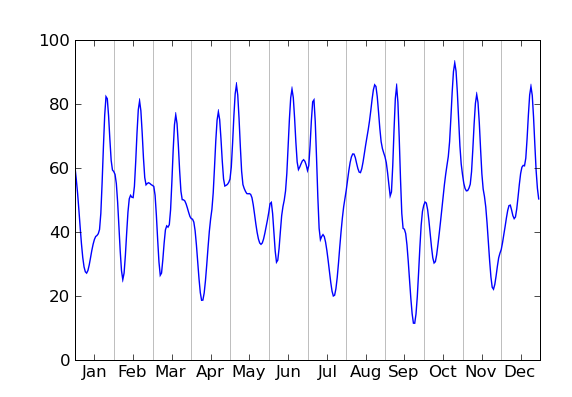
\includegraphics[width=\textwidth]{figures/conditions-a.png}
                \caption{An ordered line chart.}
                \label{fig:avg_line}
        \end{subfigure}
        \begin{subfigure}[b]{0.45\textwidth}
                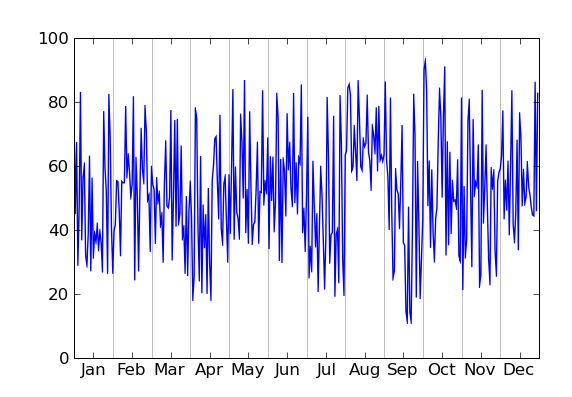
\includegraphics[width=\textwidth]{figures/conditions-b.png}
                \caption{A 1D permuted line chart}
                \label{fig:avg_line_p}
        \end{subfigure}
        \\
        \begin{subfigure}[b]{0.45\textwidth}
                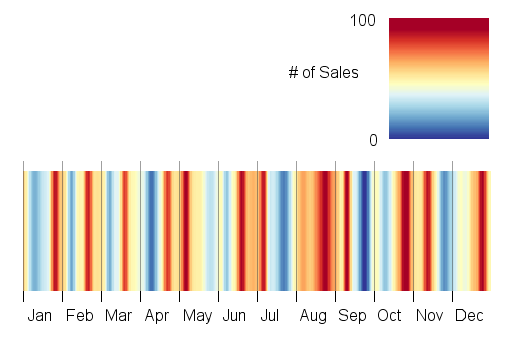
\includegraphics[width=\textwidth]{figures/conditions-c.png}
                \caption{An ordered colorfield.}
                \label{fig:avg_color}
        \end{subfigure}
        \begin{subfigure}[b]{0.45\textwidth}
                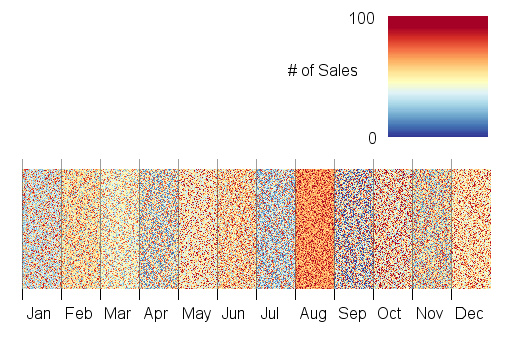
\includegraphics[width=\textwidth]{figures/conditions-d.png}
                \caption{A 2D permuted colorfield.}
                \label{fig:avg_color_p}
        \end{subfigure}
        \caption{Four possible visualizations for aggregate tasks \cite{correll2012}.}
        \label{fig:avg}
\end{figure}

Shneiderman's ``overview first, details on demand'' mantra \cite{shneiderman1996} was the basis of the approach taken by Correll et al.: design a visualization of aggregate data that will make use of pre-attentive processing \cite{correll2012}.  Their reasoning was that sub-ranges often need identification---e.g., which month had the highest average of sales for the company?   Therefore, Correll et al.\ proposed the use of colorfields, which use color rather than $y$-position to encode a variable, as seen in Figure~\ref{fig:avg_color}.  This was evaluated against the line chart and ``permuted'' versions of the colorfield---where the $x$- and $y$-positions of the pixels were randomly permuted within each month, seen in Figure~\ref{fig:avg_color_p}---and of the line chart---where the $x$-positions were randomly permuted within each month, seen in Figure~\ref{fig:avg_line_p}.

\begin{figure}
        \centering
        \begin{subfigure}[b]{0.4\textwidth}
                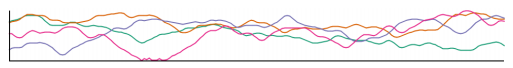
\includegraphics[width=\textwidth]{figures/ts_simplelinegraph.png}
                \caption{A simple line graph.}
                \label{fig:ts_simple}
        \end{subfigure}
        \begin{subfigure}[b]{0.4\textwidth}
                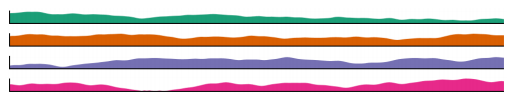
\includegraphics[width=\textwidth]{figures/ts_smallmultiples.png}
                \caption{Small multiples.}
                \label{fig:ts_smmult}
        \end{subfigure}
        \\
        \begin{subfigure}[b]{0.4\textwidth}
                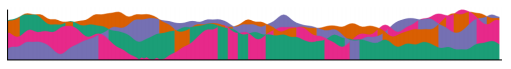
\includegraphics[width=\textwidth]{figures/ts_braidedgraph.png}
                \caption{A braided graph.}
                \label{fig:ts_braid}
        \end{subfigure}
        \begin{subfigure}[b]{0.4\textwidth}
                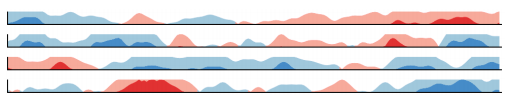
\includegraphics[width=\textwidth]{figures/ts_horizongraphs.png}
                \caption{Horizon graphs.}
                \label{fig:ts_horizon}
        \end{subfigure}
        \caption{Four possible methods for visualizing multiple time series \cite{javed2010}.}
        \label{fig:ts_compare}
\end{figure}

On the other hand, Javed et al.\ designed their alternatives with the idea that several concurrent time series often need to be viewed and compared at once \cite{javed2010}.  This can be problematic; placing all of the series on a single line chart, as in Figure~\ref{fig:ts_simple} can lead to occlusion problems, while putting each series on its own chart, also known as ``small multiples'' and seen in Figure~\ref{fig:ts_smmult}, can take a lot of screen space.  Therefore, they created a braided graph, which features all series on one chart with the coloring under the curves alternating as series intersect each other, as seen in Figure~\ref{fig:ts_braid}.  The braided graph takes a smaller amount of screen space, while each series can be distinguished by the fill coloring.  Additionally, they evaluated these three against Saito et al.'s horizon graph, as in Figure~\ref{fig:ts_horizon}, which wraps around a baseline in two color tones to save space \cite{saito2005}.

\section{Evaluations}

The goal of Correll et al.\ was to show colorfields outperform line charts for the task of finding regions of maximum averages in a series due to the pre-attentiveness and efficient perceptual averaging of color.  They ran a study using Amazon's Mechanical Turk infrastructure which asked participants to identify the month with the highest average out of a year of artificial data.  The data were produced so that the global maximum value in the data would only rarely occur in the month with the highest average, though participants were not informed of this. Answers and response times were recorded for all 74 participants.

In the other study, Javed et al.\ aimed to provide guidelines for designers wondering how to graphically present several time series given different requirements.  They ran a highly controlled user study which not only varied the four different visualization types seen in Figure~\ref{fig:ts_compare}, but also varied the number of time series (2, 4, and 8) and the total chart height (48, 96, and 192 pixels).  There were three tasks participants were asked to perform: (1) for a given time point, identify the time series with the highest value, (2) find the time series with the highest increase, and (3) given two different time points for two different series, identify which series has the highest value.  The data in the charts was randomly generated.  Answers and response times of the 16 participants were recorded.

\section{Results}

Correll et al.\ succeeded in showing that colorfields are significantly more effective than line charts for showing maximum averages.  Permuted colorfields made for slightly more accurate responses, while there was no difference between ordered and permuted line charts.  However, though response times were mentioned as recorded, there were no results, analysis, or discussion mentioned concerning time.  This is unusual considering the authors chose to use colorfields based partially on the pre-attentiveness of color.

Javed et al.\ did not find that one visualization type prevailed for all three tasks.  The simple line chart and the braided graph were best suited for local tasks, while the small multiples and horizon graphs were best for global tasks.  In general, they concluded that simple line charts and small multiples were generally more robust than horizon graphs and their newly introduced braided graphs. Additionally, they found that decreases in chart size did not affect completion time, but did decrease accuracy.  Lastly, as the number of concurrent time series increased, accuracy decreased and completion time increased. 

\section{Discussion}

\subsection{User Study}

As mentioned, Correll et al.\ used Amazon's Mechanical Turk infrastructure to conduct their study, which means users completed the trials in a browser on their own computer.  Therefore, there was no control of screen resolution, screen brightness, environmental brightness, distance of the user's eyes from the screen, and so on.  This may have had an influence---good or bad---on the experiment which cannot be deciphered in the results.  One advantage is that they were able to involve more participants than Javed et al., who used a more scientifically-controlled setting.  Some users may configure their monitors in a way which they find comfortable, leading perhaps to the best performance in the user study as possible, while other users do not even realize they can adjust their monitor, leading perhaps to worse performance at home than in scientific setting.  It is unclear which method of conducting a user study is most advantageous.

\subsection{Experiment Conditions}

The study by Correll et al.\ was relatively simple, which can be considered both good and bad.  On one hand, they completely showed what they set out to show.  On the other hand, they only varied the trials in their evaluation by the visualization method, when they could have possibly varied other properties as well.  Several lengths of time, such as 6, 12, and 24 months, or several sub-range divisions, such as 15, 30, and 60 days, could have been used to explore the effects of scaling on both time and accuracy.  Cleveland recommends a shorter chart height that makes for approximately $\pm 45 ^{\circ}$ line slopes \cite{cleveland1988}, while the charts in Figure~\ref{fig:avg} all feature large chart heights with, where applicable, more extreme slopes.  Perhaps the shape of the charts in the study should have been selected according to Cleveland's recommendation.  Alternatively, several different chart heights could have been used, which may have affected the colorfields too.  Of course, varying these additional properties would have made for more trials in the evaluation and more complicated analysis of the results, but interesting conclusions could been drawn.

Conversely, the study by Javed et al.\ was relatively complex.  Since there can be a variety of restraints and requirements in practice, this makes for results that can be meaningful for multiple applications.  However, this makes for results that are more difficult to interpret, especially since there was no clear-cut ``winner'' among the visualization types.  The authors were careful to not whole-heartedly recommend the use or avoidance of any of the types, which is perhaps not helpful for a designer seeking recommendations.  

\subsection{Tasks}

One must wonder how useful the evaluation task by Correll et al.---identifying the month with the highest average---is in reality.  Even the authors admit the task is ``contrived,'' because a chart with only the averages could have been displayed instead.  However, it is even more problematic that users may not be aware what sub-range length is relevant until they have seen the data visualized---e.g., after seeing a chart, a CEO may realize it is more important to look at three month sub-ranges over many years rather than one month sub-ranges over a single year.

For both studies, the tasks considered concern general overviews of data, rather than details.  Neither study discusses the ability of users to actually read individual values from a chart.  In fact, the charts by Javed et al.\ do not even feature labelled axes.  In practice, users may want to read values off a chart, which might prove to be quite difficult for any of the visualization types even with proper labels.  Still, perhaps users are more concerned with trends.  In this case, the study by Javed et al.\ falls short by not including any trend-based tasks.  Correll et al.\ could have included more trend-based tasks---e.g., ``Which month had the highest increase in average from the previous month?''  It would also be interesting to see how the ordered colorfield would perform in multiple series tasks such as those used by Javed et al.

\section{Conclusion}

Nobody has answered the question of whether Playfair's original line chart deserves its position as the standard mode of conveying time series data.  Javed et al.'s recommendations for a visualization are vague and suggest that a visualization should be chosen depending on the required tasks, but how often is it that only one task or one type of tasks are expected?  Correll et al. found that colorfields are better than line charts for finding maximum averages, but is this a realistic task?  It is difficult to answer these questions, and perhaps even more difficult to create generalized tasks that can easily be evaluated.  These two papers did an excellent job in accomplishing their respective purposes, but more work remains on exploring alternatives to the conventional line chart.

\bibliographystyle{plain}

\bibliography{sources}

\end{document}

